
%\marginlabel{\bf {\tt .rea} files:}
The {\tt .rea} file consists of several sections:
\subsubsection*{ Parameters and logical switches}
\begin{description}
\item{\bf parameters} These control the runtime parameters such as viscosity,
    conductivity, number of steps, timestep size, order of the timestepping,
    frequency of output, iteration tolerances, flow rate, filter strength,
    etc.   There are also a number of free parameters that the user can
    use as handles to be passed into the user defined routines in the .usr file.
\item{\bf passive scalar data} This information can be specified also in the \texttt{.uservp} routine in the .usr file. If specified in the .rea file then the coefficients for the conductivity term are listed in ascending order for passive scalars ranging \texttt{1..9} followed by the values for the $\rho c_p$ coefficients.
\begin{verbatim}
4  Lines of passive scalar data follows 2 CONDUCT; 2 RHOCP
   1.00000       1.00000       1.00000       1.00000       1.00000
   1.00000       1.00000       1.00000       1.00000
   1.00000       1.00000       1.00000       1.00000       1.00000
   1.00000       1.00000       1.00000       1.00000
\end{verbatim}
\item{\bf logicals} These determine whether one is computing a steady or unsteady
  solution, whether advection is turned on, etc.
\end{description}
\begin{comment}
           13  LOGICAL SWITCHES FOLLOW
  T     IFFLOW
  T     IFHEAT
  T     IFTRAN
  T T F F F F F F F F F IFNAV & IFADVC (convection in P.S. fields)
  F F T T T T T T T T T T IFTMSH (IF mesh for this field is T mesh)
  F     IFAXIS
  F     IFSTRS
  F     IFSPLIT
  F     IFMGRID
  F     IFMODEL
  F     IFKEPS
  F     IFMVBD
  F     IFCHAR
\end{comment}
\subsubsection*{Mesh and boundary condition info} 
\begin{description}
\item{\bf geometry} The geometry is specified in an arcane format specifying
    the $xyz$ locations of each of the eight points for each element,
    or the $xy$ locations of each of the four points for each element in 2D.
A line of the following type may be encountered at the beginning of the mesh section of the area file.    
\begin{verbatim}
3.33333       3.33333     -0.833333      -1.16667     XFAC,YFAC,XZERO,YZERO
\end{verbatim}
This part is to be read by PRENEK and provides the origin of the system of coordinates \texttt{XZERO;YZERO} as well as the size of the cartesian units \texttt{XFAC;YFAC}. This one line has no impact on the mesh as being read in NEK. 

The header of the mesh data may have the following representation
\begin{center}
\begin{verbatim} **MESH DATA** 6 lines are X,Y,Z;X,Y,Z. Columns corners 1-4;5-8
      226  3         192           NEL,NDIM,NELV
     ELEMENT           1 [    1A]    GROUP    0
     \end{verbatim}
     \end{center}
The header states first how many elements are available in total ($226$), what dimension is the the problem (here three dimensional), and how many elements are in the flow mesh ($192$). 

%\begin{center}
%     \begin{tabular}{l|l|l|l}
%  0.000000E+00 & 0.171820E+00 & 0.146403E+00 & 0.000000E+00 \\
%  0.190000E+00 & 0.168202E+00 & 0.343640E+00 & 0.380000E+00 \\
%  0.000000E+00 & 0.000000E+00 & 0.000000E+00 & 0.000000E+00 \\
%  0.000000E+00 & 0.171820E+00 & 0.146403E+00 & 0.000000E+00 \\
%  0.190000E+00 & 0.168202E+00 & 0.343640E+00 & 0.380000E+00  \\
%  0.250000E+00 & 0.250000E+00 & 0.250000E+00 & 0.250000E+00  \\
%  \end{tabular}
%\end{center}

\begin{table}
\subfloat[Descriptor]{
\begin{tabular}{l c c c c}
%\fontsize 
  $\texttt{Face \{1,2,3,4\}}$&&&&\\
  $x_{1,\ldots,4}=$& 0.000000E+00 & 0.171820E+00 & 0.146403E+00 & 0.000000E+00 \\
  $y_{1,\ldots,4}=$&0.190000E+00 & 0.168202E+00 & 0.343640E+00 & 0.380000E+00 \\
  $z_{1,\ldots,4}=$&0.000000E+00 & 0.000000E+00 & 0.000000E+00 & 0.000000E+00 \\
  $\texttt{Face \{5,6,7,8\}}$&&&&\\
  $x_{5,\ldots,8}=$&0.000000E+00 & 0.171820E+00 & 0.146403E+00 & 0.000000E+00 \\
  $y_{5,\ldots,8}=$&0.190000E+00 & 0.168202E+00 & 0.343640E+00 & 0.380000E+00  \\
  $z_{5,\ldots,8}=$&0.250000E+00 & 0.250000E+00 & 0.250000E+00 & 0.250000E+00  
  \end{tabular}} 
%\subfloat[Element]{\raisebox{-10pt}{\vspace{0.5cm}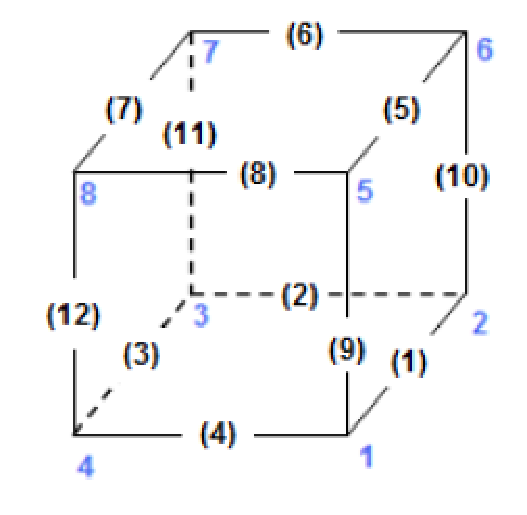
\includegraphics[scale=0.4]{Figs/3dcube}\label{fig:3dcube}}}
%{\begin{minipage}[c][1\width]{0.4\textwidth}\centering 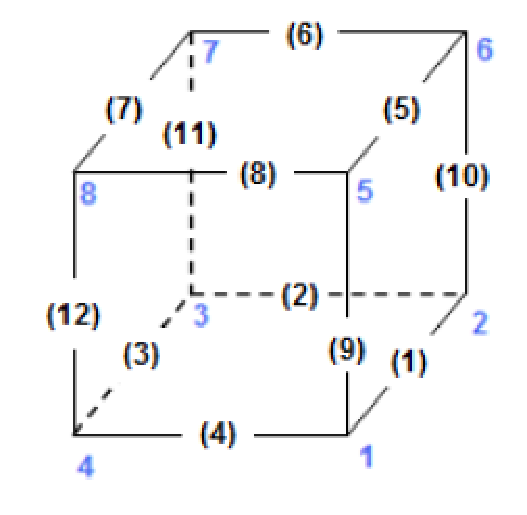
\includegraphics[width=0.4\textwidth]{Figs/3dcube} \end{minipage}}
\caption{Geometry description in .rea file}
\end{table}
\normalsize

\begin{figure}
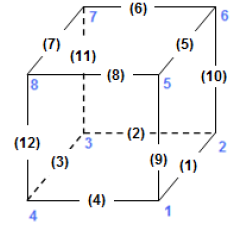
\includegraphics[scale=0.5]{Figs/3dcube.png}
\caption{Geometry description in .rea file (sketch of one element ordering)}
\end{figure}

\item{\bf curvature} 
     This section describes the deformation for elements that are curved.
     Currently-supported curved side or edge definitions include ``C''
     for circles, ``s'' for spheres, and ``m'' for midside-node positions
     associated with quadratic edge displacement. If no curved data is available the section remains empty.
     Example
     
     The section header may look like this 
     \begin{center}
     \texttt{640 Curved sides follow IEDGE,IEL,CURVE(I),I=1,5, CCURVE} 
     \end{center}
     and the data is stored as follows
  \footnotesize   
     \begin{center}
\begin{tabular}{ l|l|l|l|l }
   \hline
 \texttt{IEDGE}& \texttt{IEL} &\texttt{CURVE(12,1,IEL)} &\texttt{CURVE(12,2..5,IEL)}&\texttt{CCURVE(12,IEL)} \\ \hline \hline
  3&  1 &  1.0000  &      0.0000 &    C \\
  7 & 1 &  1.0000  &      0.0000 &    C\\
   \hline
\end{tabular}   
\end{center}
\normalsize
     The array \texttt{CCURVE} (char curve) holds a character denoting the type of curved boundary, while the array \texttt{CURVE} holds the actual information about the curved boundary. There are up to five available components in the \texttt{CURVE} array in case more information is needed by other implementations, that do not represent the default. We may have
     \begin{itemize}
     \item 'C' stands for circle and is given by the radius of the circle, thus filling in only the first component of the \texttt{CURVE(12,1,NEL)} 
     \item 'S' stands for sphere and is given by the radius and the center of the sphere, thus filling the first 4 components of the \texttt{CURVE(12,1\ldots 4,NEL)}
     \item 'M' is given by the coordinates of the midside-node, thus filling the first 3 components of the \texttt{CURVE(12,1\ldots 3,NEL)}, and leads to a second order reconstruction of the face.
     \end{itemize}
Both 'C' and 'S' types allow for a surface of as high order as the polynomial used in the spectral method, since they have an underlying analytical description, any circle arc can be fully determined by the radius and end points. However for the 'M' curved element descriptor the surface can be reconstructed only up to second order. This can be later updated to match the high-order polynomial after the GLL points have been distributed across the boundaries. In .usrdat2 the user can move the geometry to match the intended surface, followed by a call to the subroutine 'fixgeom' which can realign the point distribution in the interior of the element.

\item{\bf boundary conditions} 
     Boundary conditions (BCs) are specified for each face of each element,
     for each {\tt field} (velocity, temperature, passive scalar \#1, etc.).
     A common BC is {\tt P}, which indicates that an element face is 
     connected to another element to establish a periodic BC.   Many of the 
     BCs support either a constant specification or a user defined
     specification which
     may be an arbitrary function.   For example, a constant Dirichlet
     BC for velocity is specified by {\tt V}, while a user defined BC
     is specified by {\tt v}.   This upper/lower-case distinction is 
     used for all cases.   There are about 70 different types of boundary
     conditions in all, including free-surface, moving boundary, heat flux,
     convective cooling, etc.
     
      The section header may look like this 
     \begin{center}
     \texttt{ ***** FLUID   BOUNDARY CONDITIONS *****}

     \end{center}
     and the data is stored as follows
      \footnotesize   
     \begin{center}
\begin{tabular}{ l|l|l|l|l|l }
   \hline
 \texttt{CBC}& \texttt{IEL} &\texttt{IEDGE} &\texttt{CONN-IEL}&\texttt{CONN-IEDGE} & redundant\\ \hline \hline
  E   & 1 & 1 &  4.00000   &    3.00000  &     0.00000      \\
   ..   & .. & .. &  ..   &   .. &    ..      \\
   W  &  5 & 3 &  0.00000  &     0.00000  &     0.00000    \\
    ..   & .. & .. & ..   &   ..  &    ..      \\
   P  &  5 & 5  & 149.000 &      6.00000  &     0.00000 \\
   \hline
\end{tabular}   
\end{center}
\normalsize
     
\end{description}

\subsubsection*{ Output info} 
\begin{description}
\item{\bf restart conditions} 

     Here, one can specify a file to use as an initial condition.
     The initial condition need not be of the same polynomial order
     as the current simulation.   One can also specify that, for example,
     the velocity is to come from one file and the temperature from another.
     The initial time is taken from the last specified restart file, but 
     this can be overridden.
\item{\bf History points}

The following section defines history points in the {\tt .rea} file, see example {\tt vortex/r1854a.rea}, or {\tt shear4/shear4.rea}
\begin{verbatim}
0 PACKETS OF DATA FOLLOW\\
***** HISTORY AND INTEGRAL DATA *****\\
    56 POINTS. H code, I,J,H,IEL \\
UVWP    H     31     31   1   6\\
UVWP    H     31     31   31  6\\
UVWP    H     31     31   31  54\\
 "      "      "      "    "   "\\
\end{verbatim}

The {\tt "56 POINTS"} line needs to be followed by 56 lines of the type shown. However, in each of the following lines, which have the {\tt UVWP} etc., location is CRUCIAL, it
must be layed out exactly as indicated above\footnote{these lines contain character strings, they use formatted reads}, it is therefore advisable to refer to the examples {\tt vortex, shear4}.  If you want to pick points close to the center of element 1 and are running with lx1=10, say, you might choose {\tt UVWP H 5 5 5 1}. \footnote{the indicated point would really be at the middle of the element only if lx1=9}

The UVWP tells the code to write the 3 velocity components and pressure to the .sch file at
each timestep (or, more precisely, whenever {\tt mod(istep,iohis)=0}, where {\tt iohis=param(52))}.
Note that if you have more than one history point then they are written sequentially at each
timestep. Thus 10 steps in the first example with {\tt param(52)=2} would write {\tt (10/2)*56 = 280}
lines to the .sch file, with 4 entries per line. The "H" indicates that the entry corresponds to a requested history point. A note of caution: if the {\tt ijk} values (5 5 5 in the preceding example line) exceed {\tt lx1,ly1,lz1} of your SIZE file, then they are truncated to that value. For example, if {\tt lx1=10} for the data at the top (31 31 31) then the code will use {\tt ijk} of (10 10 10), plus the given element number, in identifying the history point. It is often useful to set {\tt ijk} to large values (i.e., > {\tt lx1}) because the endpoints of the spectral element mesh are invariant when {\tt lx1} is changed. 

\begin{comment}
7. A difficulty with the current nek history point specification is finding the requisite ijke (e=element
number) values that correlate to the point of interest. There is a way to do this in postx that
is relatively painless, but this is not useful for very large problems. (The approach is:
SET PLOT FORMAT
SCALAR
VALUES
PLOT
Follow the instructions and for each point requested, postx will write to the screen lines that
are similar to the above, ready to be pasted into the .rea file.)
8. When you run nek, it will write the coordinate information to the logfile on the first timestep
so that you can verify the point locations.
\end{comment}
\item{\bf output specifications} 
     Outputs are discussed in a separate section below.
\end{description}


\noindent
It is important to note that Nek5000 currently supports two input file
formats, ascii and binary.   The {\tt .rea} file format
described above is ascii.  For the binary format, all sections
of the .rea file having storage requirements that scale with 
number of elements (i.e., geometry, curvature, and boundary 
conditions) are moved to a second, {\tt .re2}, file and
written in binary.   The remaining sections continue to 
reside in the {\tt .rea} file.   The distinction between
the ascii and binary formats is indicated in the {\tt .rea}
file by having a negative number of elements.
There are converters, {\tt reatore2} and {\tt re2torea}, in the Nek5000
tools directory to change between formats.   The binary file
format is the default and important for {\tt I/O} performance when the
number of elements is large ( $>$ 100000, say).
